\documentclass{article}[18pt]
\usepackage{../../../../../format}
\lhead{ADS - Rob Powell}


\begin{document}
\begin{center}
\underline{\huge Recurrences}
\end{center}
\section{Intro}
We've seen two types of algorithms: iterative and recursive.
To analyse iterative algorithms,
\begin{itemize}
\item look at loop structure,
\item identify relevant operations, and
\item essentially, count them.
\end{itemize}
One often ends up with some sort of sum (the more nested
loops, the more nested sums).\\
\\
To analyse recursive algorithms, first of all note that most of them
are actually hybrids between iterative and strictly recursive (e.g., the
Partition funcion in QuickSort is iterative, the rest of QuickSort is
recursive.\\
Anyway,
\begin{itemize}
	\item Look at recursive structure, e.g. Mergesort
	\begin{itemize}
		\item Split input of size n into two halves of equal size n/2 each
		\item Independently recurse into each half
		\item merge the resulting sorted sequences
	\end{itemize}
	\item This will normally give you a recurrence, pretty much trivially:
	$$T ( n ) \leq \left\{ \begin{array} { l l } { d } & { \text { if } n \leq c , \text { for constants } c , d > 0 } \\ { \underbrace { 2 \cdot T ( n / 2 ) } _ { \text { recursions } } + \underbrace { a \cdot n } _ { \text { merging } } } & { \text { otherwise } } \end{array} \right.$$
\end{itemize}
Three methods for solving such recurrencesL
\begin{itemize}
	\item Induction (aka guess substitute and verify)
	\item Iterative substitution (spot the pattern)
	\item Master theorem
\end{itemize}
\section{Induction}
Quite simple really, only need to:
\begin{itemize}
	\item "guess" correct solution and
	\item Verify base case(s) and step
\end{itemize}
Former is art, latter is maths\\
\\
We'll normally not spend too much time on base case(s) as
when we're talking algorithms, it's quite clear that constant size
input requires some constant number of steps, full stop.\\
\\
Interesting technical bit is step (recursion as well as induction).\\
\\
Consider again the recurrence for mergesort
$$T ( n ) \leq \left\{ \begin{array} { l l } { d } & { \text { if } n \leq c , \text { for constants } c , d > 0 } \\ { \underbrace { 2 \cdot T ( n / 2 ) } _ { \text { recursions } } + \underbrace { a \cdot n } _ { \text { merging } } } & { \text { otherwise } } \end{array} \right.$$
This looks like it ought to be $T(n)=\mathcal{O}(n\log_2n)$. This is found by working backwards from a large big O until it no longer works\\
\\
Now that we've got some guess, we need to see if it's correct.\\
Recall, we guess that $T(n)\leqslant \alpha n\log_2n$ for some constant $\alpha>0$\\
\\
In the base case, the recurrence said $T(n)\leqslant d$ if $n\leqslant c$ for constants c and d. Make $\alpha$ big enough:
$$d \leq \alpha n \log _ { 2 } n \leq \alpha c \log _ { 2 } c \quad \Leftrightarrow \quad \alpha \geq \frac { d } { c \log _ { 2 } c }$$
Because of the relation between n and c, you can swap n for c in these inequalities\\
\\
As for the rest, plug our result in
$$\begin{array} { l } { T ( n ) \leq 2 T ( n / 2 ) + a n } - \text{assumption} \\ { T ( n ) \leq 2 \alpha \frac { n } { 2 } \log _ { 2 } \frac { n } { 2 } + a n }  - \text{Replace the T part with the guess}\\ { T ( n ) \leq 2 \alpha \frac { n } { 2 } \left( \log _ { 2 } ( n ) - \log _ { 2 } ( 2 ) \right) + a n } \\ { T ( n ) \leq 2 \alpha \frac { n } { 2 } \left( \log _ { 2 } ( n ) - 1 \right) + a n } \\ { T ( n ) \leq \alpha n \left( \log _ { 2 } ( n ) - 1 \right) + a n } \\ { T ( n ) \leq \alpha n \log _ { 2 } n - \alpha n + a n } \\ { T ( n ) \leq \alpha n \log _ { 2 } n \quad \text { if } \alpha n \geq a n \Leftrightarrow \alpha \geq a } - \text{Make sure last two terms are negative} \end{array}$$
Altogether, it works for any $\alpha \geq \max \left\{ \frac { d } { c \log _ { 2 } c } , a \right\} $
\subsection{What happens if you make a bad guess?}
\subsubsection{Guess too high}
The requirement $\alpha\geqslant a$ suggests that there isn't much room for (asymptotic) improvement, as both are constants\\
\\
There would be more if we had overshot our target, for example if we had guessed $T(n)\leqslant \alpha n^2$\\
Observe:
$$\begin{array} { l } { T ( n ) \leq 2 T ( n / 2 ) + a n } \\ { T ( n ) \leq 2 \alpha ( n / 2 ) ^ { 2 } + a n } \\ { T ( n ) \leq 2 \alpha n ^ { 2 } / 4 + a n } \\ { T ( n ) \leq \alpha n ^ { 2 } / 2 + a n } \\ { T ( n ) \leq \alpha n ^ { 2 } - \alpha n ^ { 2 } / 2 + a n } \end{array}$$
True whenever
$$\alpha n ^ { 2 } / 2 \geq a n \Leftrightarrow \alpha n / 2 \geq a \quad \Leftrightarrow \quad \alpha \geq 2 a / n = \Theta ( 1 / n )$$
This isn't really any restriction for a constant $\alpha$. If you see something like this, try again with smaller guess
\subsubsection{Guess too low}
On the other hand, suppose we're being greedy, and are guessing $T(n)\leqslant \alpha n$
$$\begin{array} { l } { T ( n ) \leq 2 T ( n / 2 ) + a n } \\ { T ( n ) \leq 2 \alpha n / 2 + a n } \\ { T ( n ) \leq \alpha n + a n } \end{array}$$
This is $\leqslant \alpha n$ iff $an\leqslant 0$ which isn't going to be any time soon
\section{Iterative substitution}
Expand recurrence, spot the pattern, solve algebraically\\
\\
Again for mergesort:
$$T ( n ) \leq \left\{ \begin{array} { l l } { d } & { \text { if } n \leq c , \text { for constants } c , d > 0 } \\ { \underbrace { 2 \cdot T ( n / 2 ) } _ { \text { recursions } } + \underbrace { a \cdot n } _ { \text { merging } } } & { \text { otherwise } } \end{array} \right.$$
Expand:
$$\begin{aligned} T ( n ) & \leq 2 T ( n / 2 ) + a n \\ & \leq 2 ( 2 T ( n / 4 ) + a n / 2 ) + a n = 4 T ( n / 4 ) + a n + a n \\ & = 4 T ( n / 4 ) + 2 a n \leq 4 ( 2 T ( n / 8 ) + \text { an/4 } ) + 2 a n \\ & = 8 T ( n / 8 ) + a n + 2 a n = 8 T ( n / 8 ) + 3 a n \\ & \leq 8 ( 2 T ( n / 16 ) + a n / 8 ) + 3 a n = 16 T ( n / 16 ) + a n + 3 a n \\ & = 16 T ( n / 16 ) + 4 a n \end{aligned}$$
This looks like we can do this $\log_2n$ many times, and we'll find that after i many times
\begin{itemize}
	\item First term: $2^iT(n/2^i)$
	\item Second term $ian$
\end{itemize}
Therefore after $\log_2n$ many times,
$2^{\log_2n}\cdot$ "base case value"+$\log_2(n)an=\mathcal{O}(n\log n)$
\section{Master Theorem}
Can use if the recurrence is of the form:
$$T(n) = aT(n/b) + f (n)$$
for $a\geqslant 1$ and $b>1$\\
Eg. Mergesort a=2, b=2, f(n)=an\\
Three cases:
\begin{enumerate}
	\item If $f ( n ) = O \left( n ^ { \log _ { b } ( a ) - \epsilon } \right)$ for some constant $\epsilon > 0$ then
	$T ( n ) = \Theta \left( n ^ { \log _ { b } ( a ) } \right)$
	\item If $f ( n ) = \Theta \left( n ^ { \log _ { b } ( a ) } \right)$ then $T ( n ) = \Theta \left( n ^ { \log _ { b } ( a ) } \log n \right)$
	\item If $f ( n ) = \Omega \left( n ^ { \log _ { b } ( a ) + \epsilon } \right)$ for some constant $\epsilon > 0$ and if
	af $( n / b ) \leq c f ( n )$ for some constant $c < 1$ and all $n$ large
	enough then $T ( n ) = \Theta ( f ( n ) )$
\end{enumerate}
With MergeSort, $n ^ { \log _ { b } ( a ) } = n ^ { \log _ { 2 } ( 2 ) } = n$ and $f ( n ) = a n ,$ thus case 2
applies, and we find that $T ( n ) = \Theta ( n \log n )$\\
\\
Recurrence looks like so:
$$T ( n ) \leq \left\{ \begin{array} { l l } { d } & { \text { if } n \leq c , \text { constants } c , d > 0 } \\ { T ( q ) + T ( n - q - 1 ) + a \cdot n } & { \text { for some } 0 \leq q < n } \end{array} \right.$$
Again, base case isn't going to give us any trouble\\
However, can't use expansion, and can't use Master Theorem. Not easily, anyway
\subsection{Quicksort, worst case performance}
Let $T_w(n)$ be the worst case running time of (our) QS on an input of size n. Then,
$$T _ { w } ( n ) = \max _ { 0 \leq q < n } \left\{ T _ { w } ( q ) + T _ { w } ( n - q - 1 ) \right\} + a n$$
i.e. we \textbf{maximise} over all possible partitionings (q and n-q-1)\\
\\
We guess $T_w(n)\leqslant \alpha n^2$ for some constant $\alpha>0$\\
Substitute guess into recurrence:
$$\begin{aligned} T _ { w } ( n ) & = \max _ { 0 \leq q < n } \left\{ T _ { w } ( q ) + T _ { w } ( n - q - 1 ) \right\} + \text { an } \\ & \leq \max _ { 0 \leq q < n } \left\{ \alpha q ^ { 2 } + \alpha ( n - q - 1 ) ^ { 2 } \right\} + \text { an } \\ & = \alpha \cdot \max _ { 0 \leq q < n } \left\{ q ^ { 2 } + ( n - q - 1 ) ^ { 2 } \right\} + \text { an } \end{aligned}$$
Consider the expression $q ^ { 2 } + ( n - q - 1 ) ^ { 2 }$ for $0\leqslant q< n$. It's easy to see that the expression is maximal when $q=0$ or $q=n-1$
\begin{center}
	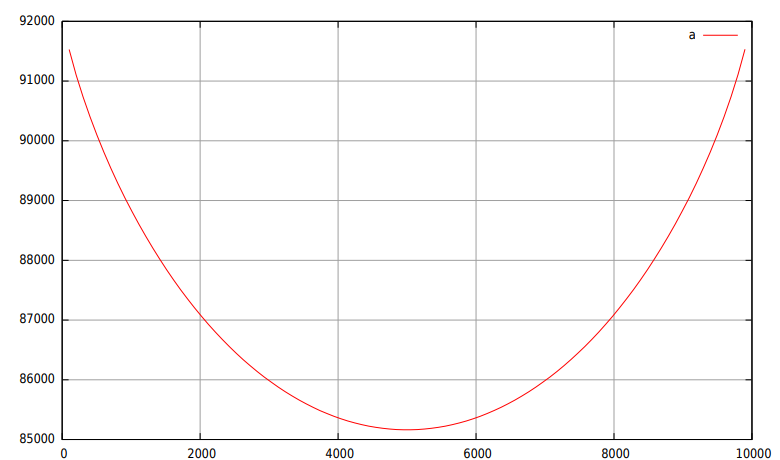
\includegraphics[scale=0.7]{Graph1}
\end{center}

\end{document}